\documentclass[tikz,border=8pt]{standalone}
% Shared look for every TikZ diagram. Load with \input{../../tools/tikz-style.tex}
\usepackage[sfdefault]{roboto}
\usetikzlibrary{arrows.meta, positioning, shapes.geometric, calc, fit, backgrounds}
\definecolor{cblue}{HTML}{4C78A8}
\definecolor{corange}{HTML}{F58518}
\definecolor{cgreen}{HTML}{54A24B}
\definecolor{cred}{HTML}{E45756}
\definecolor{cpurple}{HTML}{B279A2}
\definecolor{cgrey}{HTML}{6B6B6B}
\tikzset{
  every picture/.style={font=\sffamily, line width=1.2pt},
  box/.style={draw=#1, fill=#1!12, rounded corners=4pt, align=center, inner sep=7pt, minimum height=1.1cm},
  box/.default=cgrey,
  arrow/.style={-{Stealth[length=3mm]}, draw=cgrey, line width=1.4pt},
  title/.style={font=\sffamily\bfseries\Large},
  note/.style={font=\sffamily\small, text=cgrey, align=center},
}
\AtBeginDocument{\hyphenpenalty=10000 \exhyphenpenalty=10000}

% Direct and indirect methods (Kelly 2017, 9.4; Tedrake, Underactuated, Pontryagin's minimum principle; LaValle
% 15.2.3). Direct: discretise the problem, then optimise the numbers. Indirect: write the conditions an optimum
% must meet, then discretise and solve those.
\begin{document}
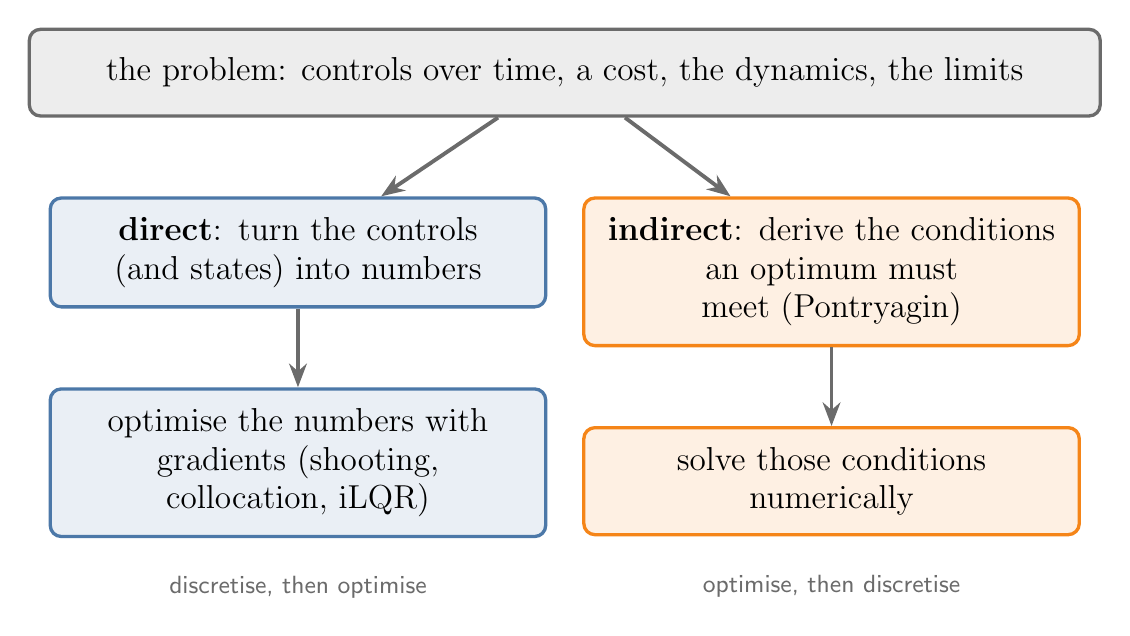
\begin{tikzpicture}[every node/.append style={font=\large}, node distance=1.0cm,
  st/.style={box=#1, minimum width=6.2cm, text width=5.8cm, minimum height=1.25cm}]
  \node[box=cgrey, minimum width=13.6cm] (p) {the problem: controls over time, a cost, the dynamics, the limits};
  \node[st=cblue, below left=1.0cm and -6.6cm of p] (d1) {\textbf{direct}: turn the controls\\ (and states) into numbers};
  \node[st=cblue, below=of d1] (d2) {optimise the numbers with\\ gradients (shooting, collocation, iLQR)};
  \node[st=corange, below right=1.0cm and -6.6cm of p] (i1) {\textbf{indirect}: derive the conditions\\ an optimum must meet (Pontryagin)};
  \node[st=corange, below=of i1] (i2) {solve those conditions\\ numerically};
  \draw[arrow] (p) -- (d1); \draw[arrow] (d1) -- (d2);
  \draw[arrow] (p) -- (i1); \draw[arrow] (i1) -- (i2);
  \node[note, below=0.35cm of d2, text width=6cm] {discretise, then optimise};
  \node[note, below=0.35cm of i2, text width=6cm] {optimise, then discretise};
\end{tikzpicture}
\end{document}
